\documentclass[]{article}
\usepackage{lmodern}
\usepackage{amssymb,amsmath}
\usepackage{ifxetex,ifluatex}
\usepackage{fixltx2e} % provides \textsubscript
\ifnum 0\ifxetex 1\fi\ifluatex 1\fi=0 % if pdftex
  \usepackage[T1]{fontenc}
  \usepackage[utf8]{inputenc}
\else % if luatex or xelatex
  \ifxetex
    \usepackage{mathspec}
  \else
    \usepackage{fontspec}
  \fi
  \defaultfontfeatures{Ligatures=TeX,Scale=MatchLowercase}
\fi
% use upquote if available, for straight quotes in verbatim environments
\IfFileExists{upquote.sty}{\usepackage{upquote}}{}
% use microtype if available
\IfFileExists{microtype.sty}{%
\usepackage{microtype}
\UseMicrotypeSet[protrusion]{basicmath} % disable protrusion for tt fonts
}{}
\usepackage[margin=1in]{geometry}
\usepackage{hyperref}
\hypersetup{unicode=true,
            pdftitle={Friend or Foe - Likelihood Ratio Tests and CIs},
            pdfborder={0 0 0},
            breaklinks=true}
\urlstyle{same}  % don't use monospace font for urls
\usepackage{graphicx,grffile}
\makeatletter
\def\maxwidth{\ifdim\Gin@nat@width>\linewidth\linewidth\else\Gin@nat@width\fi}
\def\maxheight{\ifdim\Gin@nat@height>\textheight\textheight\else\Gin@nat@height\fi}
\makeatother
% Scale images if necessary, so that they will not overflow the page
% margins by default, and it is still possible to overwrite the defaults
% using explicit options in \includegraphics[width, height, ...]{}
\setkeys{Gin}{width=\maxwidth,height=\maxheight,keepaspectratio}
\IfFileExists{parskip.sty}{%
\usepackage{parskip}
}{% else
\setlength{\parindent}{0pt}
\setlength{\parskip}{6pt plus 2pt minus 1pt}
}
\setlength{\emergencystretch}{3em}  % prevent overfull lines
\providecommand{\tightlist}{%
  \setlength{\itemsep}{0pt}\setlength{\parskip}{0pt}}
\setcounter{secnumdepth}{0}
% Redefines (sub)paragraphs to behave more like sections
\ifx\paragraph\undefined\else
\let\oldparagraph\paragraph
\renewcommand{\paragraph}[1]{\oldparagraph{#1}\mbox{}}
\fi
\ifx\subparagraph\undefined\else
\let\oldsubparagraph\subparagraph
\renewcommand{\subparagraph}[1]{\oldsubparagraph{#1}\mbox{}}
\fi

%%% Use protect on footnotes to avoid problems with footnotes in titles
\let\rmarkdownfootnote\footnote%
\def\footnote{\protect\rmarkdownfootnote}

%%% Change title format to be more compact
\usepackage{titling}

% Create subtitle command for use in maketitle
\newcommand{\subtitle}[1]{
  \posttitle{
    \begin{center}\large#1\end{center}
    }
}

\setlength{\droptitle}{-2em}

  \title{Friend or Foe - Likelihood Ratio Tests and CIs}
    \pretitle{\vspace{\droptitle}\centering\huge}
  \posttitle{\par}
    \author{}
    \preauthor{}\postauthor{}
    \date{}
    \predate{}\postdate{}
  

\begin{document}
\maketitle

\subsection{Set Up/Reminder of Example}\label{set-upreminder-of-example}

Recall the friend or foe example: 16 ten month old babies were shown a
sequence of videos where a helpful toy assisted a character in going up
a hill, or an unhelpful toy pushed the character down the hill. In the
experiment, \(x = 14\) out of 16 babies chose the helpful toy to play
with when given a choice.

\(X \sim \text{Binomial}(16, \theta)\)

\subsection{1. Likelihood Ratio Test}\label{likelihood-ratio-test}

Let's conduct a test of the claim that ten month old babies are not
capable of processing the contents of the video; they choose their toy
at random.

\(H_0: \theta = 0.5\)

\(H_A: \theta \neq 0.5\)

\paragraph{\texorpdfstring{(a) Write down the form of the likelihood
ratio statistic for this test. Your answer should only involve the
random variable \(X\) and numbers, but you do not need to simplify your
expression other than any clear
cancellations.}{(a) Write down the form of the likelihood ratio statistic for this test. Your answer should only involve the random variable X and numbers, but you do not need to simplify your expression other than any clear cancellations.}}\label{a-write-down-the-form-of-the-likelihood-ratio-statistic-for-this-test.-your-answer-should-only-involve-the-random-variable-x-and-numbers-but-you-do-not-need-to-simplify-your-expression-other-than-any-clear-cancellations.}

\vspace{6cm}

\paragraph{(b) Find the observed value of the likelihood ratio
statistic. (You may want to use R to do your
calculations.)}\label{b-find-the-observed-value-of-the-likelihood-ratio-statistic.-you-may-want-to-use-r-to-do-your-calculations.}

\vspace{3cm}

\paragraph{\texorpdfstring{(c) Using a large-sample approximation to the
sampling distribution of the likelihood ratio statistic, find the
p-value for this test. (You will need to use R to do this, using one of
the \texttt{pchisq} or \texttt{qchisq}
functions.)}{(c) Using a large-sample approximation to the sampling distribution of the likelihood ratio statistic, find the p-value for this test. (You will need to use R to do this, using one of the pchisq or qchisq functions.)}}\label{c-using-a-large-sample-approximation-to-the-sampling-distribution-of-the-likelihood-ratio-statistic-find-the-p-value-for-this-test.-you-will-need-to-use-r-to-do-this-using-one-of-the-pchisq-or-qchisq-functions.}

\newpage

\subsection{2. Approximate Confidence Interval by Inverting the
Likelihood Ratio
Test}\label{approximate-confidence-interval-by-inverting-the-likelihood-ratio-test}

\paragraph{\texorpdfstring{(a) Suppose you were conducting a likelihood
ratio test of the null hypothesis \(H_0: \theta = \theta_0\) with a
significance level of \(\alpha = 0.05\). For what values of the
likelihood ratio statistic would you reject the null hypothesis? This
will be in terms of a critical value for the test, \(w^*\). What is
\(w^*\)? (You will need to use R to find this, using one of the
\texttt{pchisq} or \texttt{qchisq}
functions.)}{(a) Suppose you were conducting a likelihood ratio test of the null hypothesis H\_0: \textbackslash{}theta = \textbackslash{}theta\_0 with a significance level of \textbackslash{}alpha = 0.05. For what values of the likelihood ratio statistic would you reject the null hypothesis? This will be in terms of a critical value for the test, w\^{}*. What is w\^{}*? (You will need to use R to find this, using one of the pchisq or qchisq functions.)}}\label{a-suppose-you-were-conducting-a-likelihood-ratio-test-of-the-null-hypothesis-h_0-theta-theta_0-with-a-significance-level-of-alpha-0.05.-for-what-values-of-the-likelihood-ratio-statistic-would-you-reject-the-null-hypothesis-this-will-be-in-terms-of-a-critical-value-for-the-test-w.-what-is-w-you-will-need-to-use-r-to-find-this-using-one-of-the-pchisq-or-qchisq-functions.}

\vspace{2cm}

\paragraph{(b) Illustrate how a confidence interval could be obtained by
inverting the likelihood ratio
test.}\label{b-illustrate-how-a-confidence-interval-could-be-obtained-by-inverting-the-likelihood-ratio-test.}

Here is a plot of the likelihood function for \(\theta\):

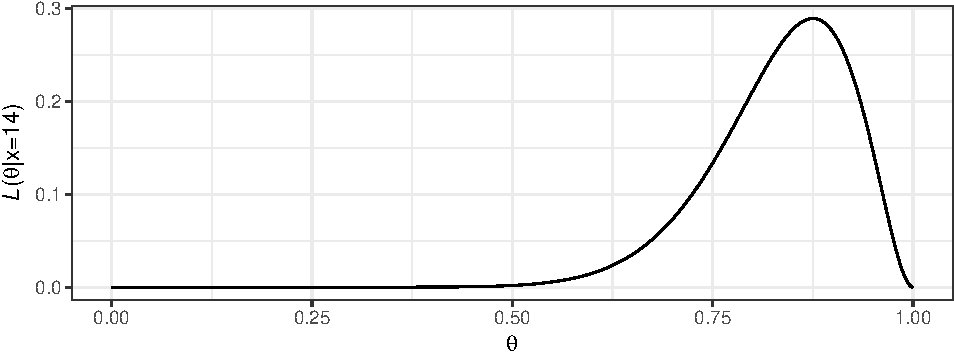
\includegraphics{20180419_LRT_CI_files/figure-latex/unnamed-chunk-3-1.pdf}

Here is a plot of the likelihood function for \(\theta\), but scaled by
dividing by the value of the likelihood function at its maximum:

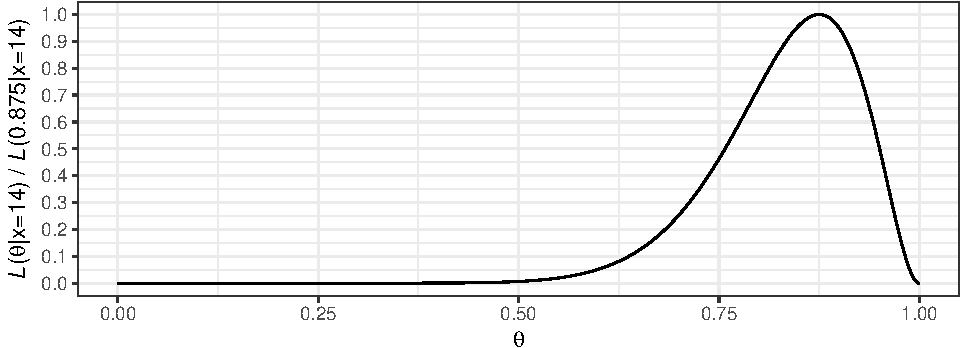
\includegraphics{20180419_LRT_CI_files/figure-latex/unnamed-chunk-4-1.pdf}

\begin{itemize}
\tightlist
\item
  On one of the two figures above (which one?), draw a line at the
  critical value \(w^*\) from part (a) (approximately - this does not
  need to be exact).
\item
  Using that line as a reference, indicate the values \(\theta_0\) for
  which you would reject the null hypothesis that \(\theta = \theta_0\).
\item
  Now indicate the values of \(\theta\) that would fall in an
  approximate 95\% confidence interval for \(\theta\) obtained by
  inverting the likelihood ratio test.
\end{itemize}

\paragraph{(c) Find the endpoints of your confidence interval using
R.}\label{c-find-the-endpoints-of-your-confidence-interval-using-r.}

Doing this exactly would require finding the roots of a degree 16
polynomial in \(\theta\). You can do that if you want, but an
approximate approach that's good enough would be to calculate the
likelihood ratio statistics at a grid of possible values for \(\theta\)
between 0 and 1, and then find out which values of \(\theta\) are in
your interval by comparing to the critical value \(w^*\).


\end{document}
